\begin{history}

    Auch über die zwei letzten Jahrzehnte hinweg spielte die Musikgesellschaft
    Hildisrieden eine zentrale Rolle im musikalischen und gesellschaftlichen
    Leben des Dorfes. Von den traditionellen Anfängen mit dem Zunftbot am
    Jahresbeginn bis zu den festlichen Jahreskonzerten, prägte die Gesellschaft
    die lokale Kultur tiefgehend. Ihre Konzerte, jedes Jahr unter einem neuen
    Motto, waren nicht nur musikalische, sondern auch gesellschaftliche
    Highlights, die Jung und Alt zusammenbrachten.

    Die Teilnahme an Musikfesten bot der Musikgesellschaft Gelegenheiten, ihre
    musikalischen Fähigkeiten unter Beweis zu stellen und Erfolge zu feiern,
    während gemeinschaftliche Konzerte und Vorbereitungen auf solche Ereignisse
    den Austausch und die Verbundenheit mit anderen Musikvereinen förderten.

    Ein besonderes Augenmerk legte die Gesellschaft auf die Pflege der
    Gemeinschaft und Kameradschaft, was sich in den gemeinsamen Ausflügen und
    Reisen zeigte. Hier ragt besonders die Reise ins Südtirol im Jahr 2002
    heraus, wo Musik, Natur und Geselligkeit im Vordergrund standen. Die
    dreitägige Tour ins Welschland 2007 bot den Musikanten nicht nur kulturelle
    Einblicke, sondern auch unvergessliche Erlebnisse.

    Ein Höhepunkt der jüngeren Vereinsgeschichte war die Ausrichtung des
    Musiktages 2013 in Hildisrieden, ein Ereignis, das die Musikgesellschaft als
    festen Bestandteil der regionalen Blasmusikszene etablierte. Die
    erfolgreiche Organisation dieses Grossereignisses war ein Beweis für das
    Engagement und die Kompetenz der Mitglieder.

    Ein weiterer herausragender Moment war die Jubiläumsreise nach London im
    Jahr 2014, anlässlich des 140-jährigen Bestehens der Musikgesellschaft. Der
    Besuch des Britischen Brass Band-Wettbewerbs in der Royal Albert Hall bot
    den Musikanten nicht nur musikalische Inspiration, sondern auch die
    Gelegenheit, die kulturellen Sehenswürdigkeiten Londons zu erkunden. Diese
    Reise hinterliess bleibende Eindrücke bei jedem Teilnehmenden.

    Im Juni 2021 erhielt die Musikgesellschaft Hildisrieden nach 28 Jahren neue
    Uniformen. Die Neuuniformierung wurde trotz pandemiebedingter
    Einschränkungen feierlich zelebriert.

    Neben diesen besonderen Anlässen ist die Musikgesellschaft auch im täglichen
    Dorfleben aktiv, gestaltet kirchliche und gesellschaftliche Feste mit und
    setzt sich für die musikalische Jugendförderung ein. Durch diese
    vielfältigen Aktivitäten beweist die Musikgesellschaft Hildisrieden auch in
    jüngerer Zeit ihre musikalische Vielseitigkeit, ihr Engagement für die
    Gemeinschaft und ihre Leidenschaft für die Musik.

    \subsubsection*{Eidg. Musikfest Fribourg 2001}

    Anfang Juni führte die MGH gemeinsam mit der Feldmusik Hellbühl und
    Feldmusik Neuenkirch ein Vorbereitungskonzert im Inpuls durch, das bei
    vielen Besuchern für Begeisterung sorgte.

    Wenige Tage später, am 16. und 17. Juni, begaben sich die Musikanten trotz
    regnerischem Wetter in bester Stimmung nach Fribourg. Dort absolvierten sie
    im Platzregen stehend ihren Marschmusikvortrag und erreichten mit 103
    Punkten eine Platzierung in der oberen Ranglistenhälfte.

    Die Vorbereitung auf die Konzertstücke \enquote{Alpine Variations} von
    Bertrand Moren und \enquote{Prelude and Celebration} von James Curnow zahlte
    sich aus, denn beide Darbietungen überzeugten die Jury und bescherten der
    Musikgesellschaft mit je 150 Punkten den 19. Rang unter 46 teilnehmenden
    Vereinen.

    Der Ausflug endete mit einer Erkundung der Altstadt von Fribourg und am
    Sonntag mit einem herzlichen Empfang durch die Hildisrieder Bevölkerung.

    \subsubsection*{Reise ins Südtirol 2002}
    Während ihrer dreitägigen Reise ins Südtirol erlebte die Musikgesellschaft
    Hildisrieden neben musikalischen Darbietungen und kulturellen Ausflügen auch
    heitere Momente.

    Gleich nach ihrer Ankunft und dem Beziehen der Zimmer fanden einige der
    jüngeren Mitglieder Gelegenheit für eine aussergewöhnliche Aktion am Pool.
    Getrieben von jugendlicher Ausgelassenheit, wagten sie es, nicht einfach nur
    in den Pool zu springen, sondern vollführten den Sprung gemeinsam mit einem
    Gartenstuhl ins erfrischende Wasser.

    Am nächsten Tag stand der Besuch eines Weinguts in Kaltern auf dem Programm,
    gefolgt von einer Wanderung, Baden und Zeit zur freien Entspannung. Der
    Abend wurde mit einem Kurkonzert in Eppan abgerundet, trotz einiger
    Herausforderungen durch den Wind.

    \begin{MulticolFigure}
        \centering
        \includegraphics[width=0.93\linewidth]{./chap/2001-2024/2002/MGH-Südtirol-2002-3.jpg}
        \captionof{figure}{Konzert mit Windstörungen in Eppan}
    \end{MulticolFigure}

    \begin{MulticolFigure}
        \centering
        \includegraphics[width=0.93\linewidth]{./chap/2001-2024/2002/MGH-Südtirol-2002-1.jpg}
        \captionof{figure}{Die jüngeren der Reisegruppe}
    \end{MulticolFigure}

    Den Abschluss der Reise bildete ein Frühschoppenkonzert in St. Maria, bevor
    es zurück nach Hildisrieden ging.

    \subsubsection*{Musikreise in die Freiberge, 2004}

    Am 4. und 5. September 2004 unternahmen wir einen Ausflug in den Jura. Der
    Samstag begann früh mit der Abfahrt, gefolgt von einer Mittagspause, bevor
    wir in Bassecourt ankamen. Hier erwartete die Teilnehmer eine spannende
    Fahrt mit einer Privatbahn aus dem Jahr 1935.

    \begin{MulticolFigure}
        \centering
        \includegraphics[width=0.7\linewidth]{./chap/2001-2024/2004/musikreise2004_03.jpg}
    \end{MulticolFigure}

    Die Reise nahm eine überraschende Wendung, als die Bahn unterwegs von drei
    \enquote{bewaffneten} Cowboys gestoppt wurden, die Hildegard und Urs als
    Geiseln mitnahmen. Nachdem der Tuba-Franz das Lösegeld aufgetrieben hatte,
    setzte die Reisegruppe die Fahrt fort und erreichte Saignelegier, wo im
    Hotel eincheckt wurde.

    Der nächste Tag führte uns zum Fluss Le Doubs. Nach einem kurzen Spaziergang
    erreichten wir die Doubsfälle und genossen eine Schifffahrt, die auch zur
    geschichtlichen Bildung beitrug. Nach dem Mittagessen trat die Reisegruppe
    die Heimreise über Biel an.

\end{history}

\subsection*{Eidg. Musikfest Luzern 2006}

\begin{history}

    Am 17. und 18. Juni fand das Eidgenössische Musikfest in Luzern statt, und
    die Musikgesellschaft Hildisrieden startete den Tag frühmorgens mit einem
    gemeinsamen Frühstück, das der Wirt des Restaurants Chrüz sponserte. Nachdem
    alle gestärkt waren, machten wir uns mit dem Bus auf den Weg nach Luzern.

    \begin{MulticolFigure}
        \centering
        \includegraphics[width=0.7\linewidth]{./chap/2001-2024/2006/Mentale-Einstimmung.jpg}
        \captionof{figure}{Mentales Training}
    \end{MulticolFigure}

    In der Bruchmattturnhalle eröffneten wir als erste in der 2. Klasse Brass
    Band den Konzertmorgen mit dem Pflichtstück \enquote{Fanfare and Funk} und
    erzielten 258 Punkte. Sicherlich auch für die Juroren ungewohnt war, dass
    bei uns eine Bassgitarre für funkige Klänge sorgte.

    Anschliessend spielten wir unser Selbstwahlstück \enquote{Dimensions}, für
    das wir 245 Punkte erhielten, was uns insgesamt auf den 14. Platz mit 503
    Punkten brachte.

    \begin{MulticolFigure}
        \centering
        \includegraphics[width=0.93\linewidth]{./chap/2001-2024/2006/Marschmusik.jpg}
    \end{MulticolFigure}

    Unser Auftritt in der Marschmusik auf der Luzerner Haldenstrasse mit dem
    Marsch \enquote{Triumph} war besonders erfolgreich: mit 253 Punkten
    erreichten wir den hervorragenden 4. Platz.

    \vfill
    \columnbreak

    \subsubsection*{3-tägige Musigreise in die Romandie, August 2007}

    In Wasen im Emmental wurde um 10 Uhr der erste Kaffee-Halt gemacht. Beim
    Hornussen zeigte sich schon bald mal, welche Talente sich wirklich hinter
    den Musikanten verstecken.

    \begin{MulticolFigure}
        \centering
        \includegraphics[width=0.93\linewidth]{./chap/2001-2024/2007/Max-am-Hornussen.JPG}
        \captionof{figure}{Am Vormittag Hornussen}
    \end{MulticolFigure}

    Gegen Mittag machte die Reisegesellschaft dann in Niede\emph{rösch} halt, um
    sich für einen strengen Nachmittag zu stärken. Von unserem Dirigenten fehlte
    trotz Dorfnamen jede Spur.

    Danach nahm man Fahrt Richtung Ligerz (BE), dem \enquote{Dorf am
        Röschtigraben}. Nach einem intensiven, viertelstündigen Aufstieg wurden
    die Musikanten beim Weinbau \enquote{Festiguet} von Rolf Teutsch
    empfangen. Die anschliessende Weinbaubesichtigung rückte dabei etwas in
    den Hintergrund, dafür gestaltete sich die Weindegustation umso länger.
    Gemäss Prophezeiungen des Weinbauers sollten die Musikanten nach dieser
    rund zweistündigen Degustation nicht nur die wunderbare Aussicht auf den
    Bielersee geniessen dürfen, sondern sogar das Dach Afrikas, den
    Kilimandscharo, entdecken. Nicht zum letzten Mal auf dieser dreitägigen
    Reise, wie sich herausstellte.

    \begin{MulticolFigure}
        \centering
        \includegraphics[width=0.93\linewidth]{./chap/2001-2024/2007/Weindegu.JPG}
        \captionof{figure}{Am Nachmittag Wein degustieren}
    \end{MulticolFigure}


    Nach der Fahrt nach Murten und einem feinen Nachtessen durfte die Zeit jeder
    selber nutzen, mehr oder weniger lang Murten auszukundschaften.

    Früh am Samstagmorgen (10.15 Uhr) fuhr die Reisetruppe dann weiter mit
    Reiseziel Le Pont am Lac de Joux. Nach einer Mittagspause zeigte sich die
    MGH mit einer zweistündigen Wanderung zu den Grotten von Vallorbe (VD) von
    ihrer sportlichen Seite. Selbstverständlich durfte auch die Besichtigung der
    Grotten nicht fehlen. Bei etwas kühleren Temperaturen von rund 10 Grad
    zeigte der Führer die Attraktionen dieser Grotte, die seit 1974 öffentlich
    zugänglich ist.

    Der Abend wurde dann in der \enquote{olympischen Stadt} Lausanne verbracht.
    Beim gemeinsamen Nachtessen im \enquote{Ticino de Lausanne} und dem Besuch
    der ortsansässigen Brasserie wurde der Abend um die Ohren geschlagen.
    Anscheinend hat die Wanderung aber bei einigen Musikanten zu wenig gewirkt.
    Gerüchteweise soll die Nacht plötzlich sehr kurz und sogar noch Berge namens
    Kilimandscharo nach Lausanne verschoben worden sein. Die eingetragene
    Nachtruhe um 22:00 wurde von der Reiseleitung höchstpersönlich um mehrere
    Stunden hinausgezögert, schliesslich ist man nur einmal in Lausanne.

    Sonntags wollte die Reisegruppe die sicherlich wunderbare und einzigartige
    Aussicht von der Turmspitze der Kathedrale in Lausanne geniessen. Doch des
    einen Leid, war des anderen Freud: Die Turmspitze kann an Tagen wie diesen
    nur ab 14 Uhr bezwungen werden. Einigen fiel wohl ein Stein vom Herzen. So
    reiste die MGH unverrichteter Dinge (ein paar Gebete ausgenommen) weiter
    Richtung Montreux. Ein Teil der Gruppe erkundete Montreux, während dem die
    anderen im Aquaparc das Vergnügen suchten. Im späteren Nachmittag wurden
    dann alle wieder "zusammengesammelt". Auf dem Heimweg versuchten viele, die
    Musigreise bei einem Nickerchen nochmals zu Gemüte zu führen. Kurz vor 19
    Uhr trafen die Musikanten unversehrt in Hildisrieden ein.


    \subsubsection*{Oberwalliser Musikfest Susten-Leuk, 13. Juni 2009}

    Beim Oberwalliser Musikfest erlebte unsere Musikgesellschaft eine
    unvergessliche Erfahrung. Die Darbietung der Marschmusik begann wie für uns
    üblich mit Tambour-Beginn, Spiel vom Marsch \enquote{Fanfare en Fête} von
    Jean-Pierre Fleury und anschliessendem Spiel-Halt. Doch an diesem Tag lief
    es anders als erwartet.

    Die Walliser Zuschauer, die sich entlang der Strecke versammelt hatten,
    standen noch immer da, Hunderte Meter weiter, links und rechts der Parade.
    Sie erwarteten offensichtlich mehr von uns, und so, getrieben von ihrer
    ungeduldigen Anteilnahme, formierten wir uns erneut und wiederholten
    denselben Marsch sicher noch drei Mal.

    Nachdem die Marschmusik schliesslich zum Abschluss gekommen war, widmeten
    wir uns den Konzertstücken. Für das Selbstwahlstück   \enquote{Music for a
        Festival} von Philip Sparke bekamen wir von der Jury 271 Punkte, für das
    Aufgabenstück \enquote{A Scots Miscelany} von Alan Fernie 258 Punkte.

    Obwohl wir als ausserkantonaler Verein nicht offiziell rangiert wurden,
    hätte unsere Leistung für einen stolzen 5. Rang gereicht. Diesen Erfolg
    feierten wir ausgelassen mit einem selbstmitgebrachten Pokal, zusammen mit
    der Musikgesellschaft Oberkirch, die auch mit Michael Rösch als Dirigenten
    am Musikfest teilgenommen hatte.

    Die Feierlichkeiten zogen sich bis tief in die Nacht hinein und fanden ihren
    Höhepunkt in der Zivilschutzunterkunft, die unter der ausgelassenen Stimmung
    ein wenig zu leiden hatte. Doch die unvergesslichen Momente und die
    herzliche Gastfreundschaft der Walliser machten dieses Musikfest zu einem
    prägenden Erlebnis für jeden von uns.

\end{history}

\subsection*{Kant. Musikfest Willisau 2010}

\begin{history}

    Am 6. Juni fand in Oberkirch das Vorbereitungskonzert für das Kant.
    Musikfest in Wilisau statt. Im gut gefüllten Saal fand der erste Ernstfall
    statt.

    Der Festtag begann mit der Ankunft in Willisau, wo die Musikgesellschaft
    Hildisrieden, begleitet von zwei charmanten Ehrendamen, freundlich empfangen
    wurde. Nach einem Fototermin, bei dem alle versuchten, ihre beste Seite zu
    zeigen, stärkte sich die Gruppe im Restaurant Schlossfeld mit einer üppigen
    Portion Spaghetti, was später bei der Marschmusik zu einigen
    Bewegungsproblemen führte.

    \begin{MulticolFigure}
        \centering
        \includegraphics[width=0.93\linewidth]{./chap/2001-2024/2010/MGH-Marschmusik-Willisau-2010.jpg}
    \end{MulticolFigure}

    Die MGH eröffnete den Marschmusikwettbewerb mit dem Marsch \enquote{Fanfares
        en Fête}, was den kürzeren Beinen einiger Mitglieder aufgrund des
    schnellen Tempos Herausforderungen bescherte. Wir erzielten 45.5 von 60
    möglichen Punkten und landeten auf dem 27. Platz unter 36 teilnehmenden
    Vereinen.


    Der Aufstieg zum Konzertlokal erwies sich mit etwa 300 Treppenstufen als
    besonders anstrengend. Nach einer kurzen Erholung begann um 15:40 Uhr das
    Einspielen, gefolgt von den Vorträgen. Auf der warmen Bühne präsentierten
    sie zunächst das Pflichtstück \enquote{Symphonic Contrasts} von Etienne
    Crausaz und anschliessend das Selbstwahlstück \enquote{The Prizewinners} von
    Philip Sparke. Die Musikanten und ihr Dirigent Michael Rösch waren mit ihrer
    Darbietung zufrieden und hofften auf eine gute Bewertung.

    Nach den musikalischen Anstrengungen widmete man sich der Geselligkeit.
    Einige verbrachten die Zeit bei gemütlichem Zusammensein, andere verfolgten
    den WM-Match, während die Jugendlichen ausgelassen zu irischer Musik
    tanzten.

    Bei der Mitternachtsverkündung erfuhr wir, dass wir auf dem 20. Platz unter
    26 Mitbewerbern gelandet waren. Anschliessend wurde der  Jurybericht
    genauestens studiert, um den Grund für diesen enttäuschenden Rang
    herauszufinden.

    Trotz dieses Resultats wurde natürlich bis tief in die Nacht gefeiert und in
    Gedanken die Rangliste ganz einfach umgedreht, um die MGH auf dem 7. Rang zu
    sehen und sich somit trotzdem als kleine \enquote{Prizewinner-lis} zu
    fühlen…

\end{history}

\groupphoto{0.96}{0.85}{./chap/2001-2024/2010/MGH-2010.jpg}
{\emph{Kant. Musikfest Willisau 2010}\\
    1. Reihe:\\
    Maja Achermann, Beat Koller, Markus Banz, Mathias Niggli, Martin Estermann,
    Josef Wolf, Michael Rösch, Christoph Erni, Franz Dörig, Martin Aregger,
    Silvia Schurtenberger\\
    2. Reihe:\\
    Christoph Schneider, Fabian Hüsler, Stephan Wolf, Benedikt Troxler, Urs
    Niederberger, Beat Disler, Markus Käppeli, Martin Troxler\\
    3. Reihe:\\
    Toni Bachmann, Peter Fleischli, Marina Büchler, Daniel Fleischli, Severin
    Pfister, Stefan Barmet, Dario Fleischli, Beat Bachmann, Christoph Troxler,
    Roland Klaus\\
    4. Reihe:\\
    Stephan Schneider, Peter Estermann, Armin Schmid, Franz Erni, Alexander
    Troxler, Roger Wermelinger, Mathias Rub, Manuel Andermatt } {fig:mgh-2010}


\subsection*{Musiktag Hildisrieden 2013}

\begin{history}

    \begin{wrapfigure}{r}{0.2\linewidth}
        \includegraphics[width=\linewidth]{./chap/2001-2024/2013/Musiktag-Logo.jpg}
    \end{wrapfigure}

    Der Werdegang des Musiktages 2013 in Hildisrieden begann im Herbst 2009 an
    einer ausserordentlichen GV. Für die erfolgreiche Organisation des Events
    wurde Jakob Estermann als OK-Präsident gewählt.

    Unterstützt wurde er von einem kompetenten Team, bestehend aus Christoph
    Erni als Vize-OK-Präsident und Erwin Bieri, der den Rechtsdienst übernahm.
    Sandra Bründler kümmerte sich um das Sekretariat, während Christoph Troxler
    für Musik und Anlässe zuständig war. Die Kommunikation lag in den Händen von
    Eva Arnet, und Erwin Wolf verantwortete die Festwirtschaft. Thomas Estermann
    übernahm Logistik und Bau, Erika Estermann-Disler war für personelle
    Angelegenheiten zuständig und Pirmin Furrer verwaltete die Finanzen des
    Musiktages.

    Diese Bereichsleiter wurden unterstützt von einem erweiterten OK von über 40
    Mitgliedern.

    \begin{MulticolFigure}
        \centering
        \includegraphics[width=0.93\linewidth]{./chap/2001-2024/2013/Bau-Marschmusikstrecke.jpg}
        \captionof{figure}{Aufbau des Wegs zum Start der Marschmusikstrecke}
    \end{MulticolFigure}

    Schon an der Chilbi Ende April begann die Werbung für den Musiktag, wobei
    unser Stand von vielen Besuchern frequentiert wurde. Anfang Mai fand im
    Gasthaus Löwen ein spezieller Anlass für die Gönner des Musiktages statt.
    Die musikalische Umrahmung übernahmen die Ronspatzen.

    Nur zwei Wochen später erlebten wir beim Luzerner Kantonales Jugendmusikfest
    eine unvergessliche Stimmung. 33 Jugendformationen nahmen teil. Das riesige
    Zelt auf dem Rasenplatz vibrierte während der gesamten Rangverkündigung vor
    Begeisterung.    Nach der Rangverkündigung sorgte die junge Band
    \enquote{The Fires} für Rock'n'Roll Stimmung.

    \begin{MulticolFigure}
        \centering
        \includegraphics[width=0.93\linewidth]{./chap/2001-2024/2013/Jugendmusikfest.jpg}
    \end{MulticolFigure}
    \begin{MulticolFigure}
        \centering
        \includegraphics[width=0.93\linewidth]{./chap/2001-2024/2013/Country.jpg}
    \end{MulticolFigure}

    Das Country Fest am 29. Mai zog zahlreiche Fans der Country-Musik an. Es
    wurde so intensive getanzt, dass teilweise die Konsumation etwas vergessen
    ging. Wir Musikanten und die anderen Hildisrieder Gäste sorgten jedoch für
    eine lebhafte Atmosphäre bis tief in die Nacht hinein.

    \begin{MulticolFigure}
        \centering
        \includegraphics[width=0.93\linewidth]{./chap/2001-2024/2013/Marschmusikstrecke.jpg}
    \end{MulticolFigure}

    Der Höhepunkt des Jahres war sicherlich der Luzerner Kantonale Musiktag am
    1. und 2. Juni, der trotz des schlechten Wetters am Samstag ein voller
    Erfolg wurde. 62 Musikvereine besuchten an diesem Wochenende unser Dorf.

    Das Engagement der lokalen Vereine trug zu einem reibungslosen Ablauf bei
    und machte die 12 Festlokale zu einem einmaligen Treffpunkt für alle
    Besucher. 20 Bands und Kleinformationen sorgten an beiden Wochenenden für
    beste Unterhaltung.

    \begin{MulticolFigure}
        \centering
        \includegraphics[width=0.6\linewidth]{./chap/2001-2024/2013/Unterwegs-zum-Start.jpg}
        \captionof{figure}{Unterwegs zum Marschmusikstart}
    \end{MulticolFigure}


    Die Marschmusik konnte leider nur am Sonntag stattfinden, was der Stimmung
    jedoch keinen Abbruch tat.

    \begin{MulticolFigure}
        \centering
        \includegraphics[width=0.6\linewidth]{./chap/2001-2024/2013/Showband-CH.jpg}
        \captionof{figure}{Showband.ch am Festumzug}
    \end{MulticolFigure}

    \begin{MulticolFigure}
        \centering
        \includegraphics[width=0.93\linewidth]{./chap/2001-2024/2013/Fahnendelegationen.jpg}
    \end{MulticolFigure}

    Am Sonntagnachmittag fand die Veteranenehrung mit einem festlichen Umzug mit
    vielen Fahnedelegationen statt.

    \begin{MulticolFigure}
        \centering
        \includegraphics[width=0.93\linewidth]{./chap/2001-2024/2013/MGH-Umzug.jpg}
    \end{MulticolFigure}

\end{history}

\subsection*{Jubiläumsreise nach London, 10.-13. Oktober 2014}

\begin{history}

    Anlässlich des 140-jährigen Bestehens der Musikgesellschaft Hildisrieden
    organisierte Alexander Troxler eine Reise nach London, welche von allen
    Vereinsmitgliedern bereits sehnlichst erwartet wurde.

    Am frühen Donnerstagmorgen, den 9. Oktober, besammelten sich die ersten elf
    Reiseteilnehmer auf dem Inpuls-Gelände und machten sich auf zur
    Weltmetropole London. Die restlichen 40 Reiseteilnehmer traten die
    Städtereise 24 Stunden später ebenfalls am frühen Morgen um 4.00 Uhr an.
    Nach einem sicheren und ruhigen, eineinhalb stündigen Flug ging es mit der
    U-Bahn direkt in das Zentrum der Stadt, wo ein kleiner Aufenthalt in der
    Nähe von Westminster beim \enquote{Big Ben} auf dem Programm stand.
    Anschliessend reiste die Gruppe weiter Richtung Wembley-Stadion. Am Ziel
    angelangt, wartete schon die einen Tag zuvor angereiste Truppe und die ganze
    Reisegesellschaft konnte sich zusammenfügen.

    \begin{MulticolFigure}
        \centering
        \includegraphics[width=0.93\linewidth]{./chap/2001-2024/2014/Einmarsch-Wembley.jpg}
        \captionof{figure}{Einmarsch ins Wembley Stadion}
    \end{MulticolFigure}

    Nun waren es insgesamt 51 MGHler und Angehörige der Musikgesellschaft, die
    das riesige Wembley-Stadion - ein erster Höhepunkt der Reise - vor sich
    fanden. Am Eingang des imposanten Bauwerks wurden zuerst alle Taschen und
    Jacken von Sicherheitsleuten durchsucht, bevor wir von zwei überaus
    humorvollen und freundlichen Stadionführern für den Rundgang durch das
    Stadion in Empfang genommen wurden. Nach ein paar eindrücklichen Statistiken
    rund um das Stadion wurden wir durch die Umkleideräume, Duschen,
    Fitnessräume, den Pressekonferenzraum und bis auf den Rasen geführt. 90`000
    Sitzplätze bieten jedem Besucher einen hervorragenden Blick auf das
    Spielfeld. Damit ist das Wembley eines der grössten Fussballstadien der
    Welt. Gegen den Schluss der Führung konnten wir uns sogar in die Loge der
    königlichen Familie setzen. Nach beeindruckenden und spannenden 75 Minuten
    ging die Tour zu Ende.

    \begin{MulticolFigure}
        \centering
        \includegraphics[width=0.93\linewidth]{./chap/2001-2024/2014/Wembley-Gruppe.jpg}
    \end{MulticolFigure}

    Unmittelbar neben dem Wembley Park befand sich unser Hotel. Nach dem ersten
    Besuch in der Hotelbar konnten die Zimmer bezogen werden. Der abendliche
    Ausgang war dann Sache der Reiseteilnehmer.

    Nach einem reichlichen Frühstück am Samstagmorgen war um 8.30 Uhr Besammlung
    vor dem Hotel, um zusammen zur Royal Albert Hall zu fahren. Dort fand unser
    eigentliches Reiseziel, der Final des Britischen Brass Band-Wettbewerbs
    statt. 20 Topbesetzte Bands zeigten mit dem Werk \enquote{The Legend of King
        Arthur} von Peter Meechan in diesem imposanten Konzertsaal mit rund 7‘000
    Sitzplätzen ihr Können. Die Musikanten verfolgten extrem interessiert und
    zum Teil ausgerüstet mit Partituren des Teststücks diesen Wettbewerb. Einige
    konnten es sich nicht nehmen lassen, das Teststück bis zu 18 Mal zu hören.
    Mit der weltbekannten Black Dyke Band wurde ein Favorit zum verdienten
    Sieger erklärt.

    \begin{MulticolFigure}
        \centering
        \includegraphics[width=0.93\linewidth]{./chap/2001-2024/2014/Britisch-Open-Royal-Alber-Hall.jpg}
    \end{MulticolFigure}

    Anschliessend an den Wettbewerb gab es von eben diesem britischen Meister
    noch ein Galakonzert, in dem unter anderem ein Stück aus dem letztjährigen
    Jahreskonzert der MGH aufgeführt wurde. Der anschliessende Abschluss des
    Tages war dann wiederum in eigener Organisation. Um die riesige Stadt jedoch
    noch auf eigene Faust erkunden zu können, stand am Sonntag erst am Abend der
    erste und einzige Fixtermin auf dem Reisekalender.

    Jedoch mussten die am Donnerstag angereisten Reiseteilnehmer bereits wieder
    die Heimreise antreten. Der Rest der Gesellschaft nutzte die freie Zeit
    rege, um die vielen Sehenswürdigkeiten in der Hauptstadt Englands zu
    begutachten. Unter anderem wurden die Tower Bridge, der Buckingham Palast,
    der Kensington Palast, das London Eye und nicht zuletzt \enquote{The Shard},
    ein 72-stöckiges Hochhaus mit einer eindrücklichen Aussichtsplattform auf
    250 Metern Höhe, besucht. Aber auch die gewaltigen Ausmasse der U-Bahn waren
    zum Staunen und die riesigen Einkaufsmeilen gehörten ebenfalls auf die Liste
    vieler Reiseteilnehmer.

    Nach dem gemeinsamen Nachtessen im Hotel fand der Abend an der Hotelbar
    seinen Ausklang. Und schon stand der letzte Tag der Reise vor der Tür. Nach
    dem alle Teilnehmer zusammengetrommelt waren, ging es mit vielen schönen und
    unvergesslichen Erlebnissen und Eindrücken via Flugzeug und Privatwagen
    zurück nach Hildisrieden. An dieser Stelle geht ein riesiges Dankeschön an
    unseren Posaunisten Alexander Troxler, welcher diese Jubiläums-Reise perfekt
    organisiert hatte.

\end{history}

\groupphoto{1}{1}{./chap/2001-2024/2014/Reise-Teilnehmer.jpg}
{\emph{Royal Albert Hall, London 2014}\\
} {fig:london-2014}


\subsection*{Kant. Musikfest Sempach, 6. Juni 2015}

\begin{history}


    Nach dem Probetag am 4. Juni fühlten wir uns bereit für das Fest in Sempach.
    Weil die MG Harmonie Sempach uns am Musiktag 2013 half, war es nun an uns,
    sie bei ihrem Fest entsprechend zu unterstützen. Und so arbeiteten am
    Jugendmusikfest am ersten Festwochenende die Mitglieder der MGH in Sempach
    im Service oder am Grill.

    Am zweiten Wochenende des kantonalen Musikfestes konnte endlich auch die MGH
    in die musikalischen Geschehnisse in Sempach eingreifen. Am
    Samstagnachmittag viertel vor drei standen die Musikantin und Musikanten
    unter der brütenden Sonne auf der Marschmusikstrecke bereit für die
    Parademusik mit dem Marsch \enquote{Geb. Füs. Bataillon 48}. Mit der
    kräftigen Unterstützung der mitgereisten Hildisrieder Fans gelang nach
    mehreren Jahren die Zielmarke von 50 Punkten. Diese wurde sogar um 0,6
    Punkte übertroffen, weshalb die MGH schliesslich mit dem 5. Rang belohnt
    wurde.

    \begin{MulticolFigure}
        \centering
        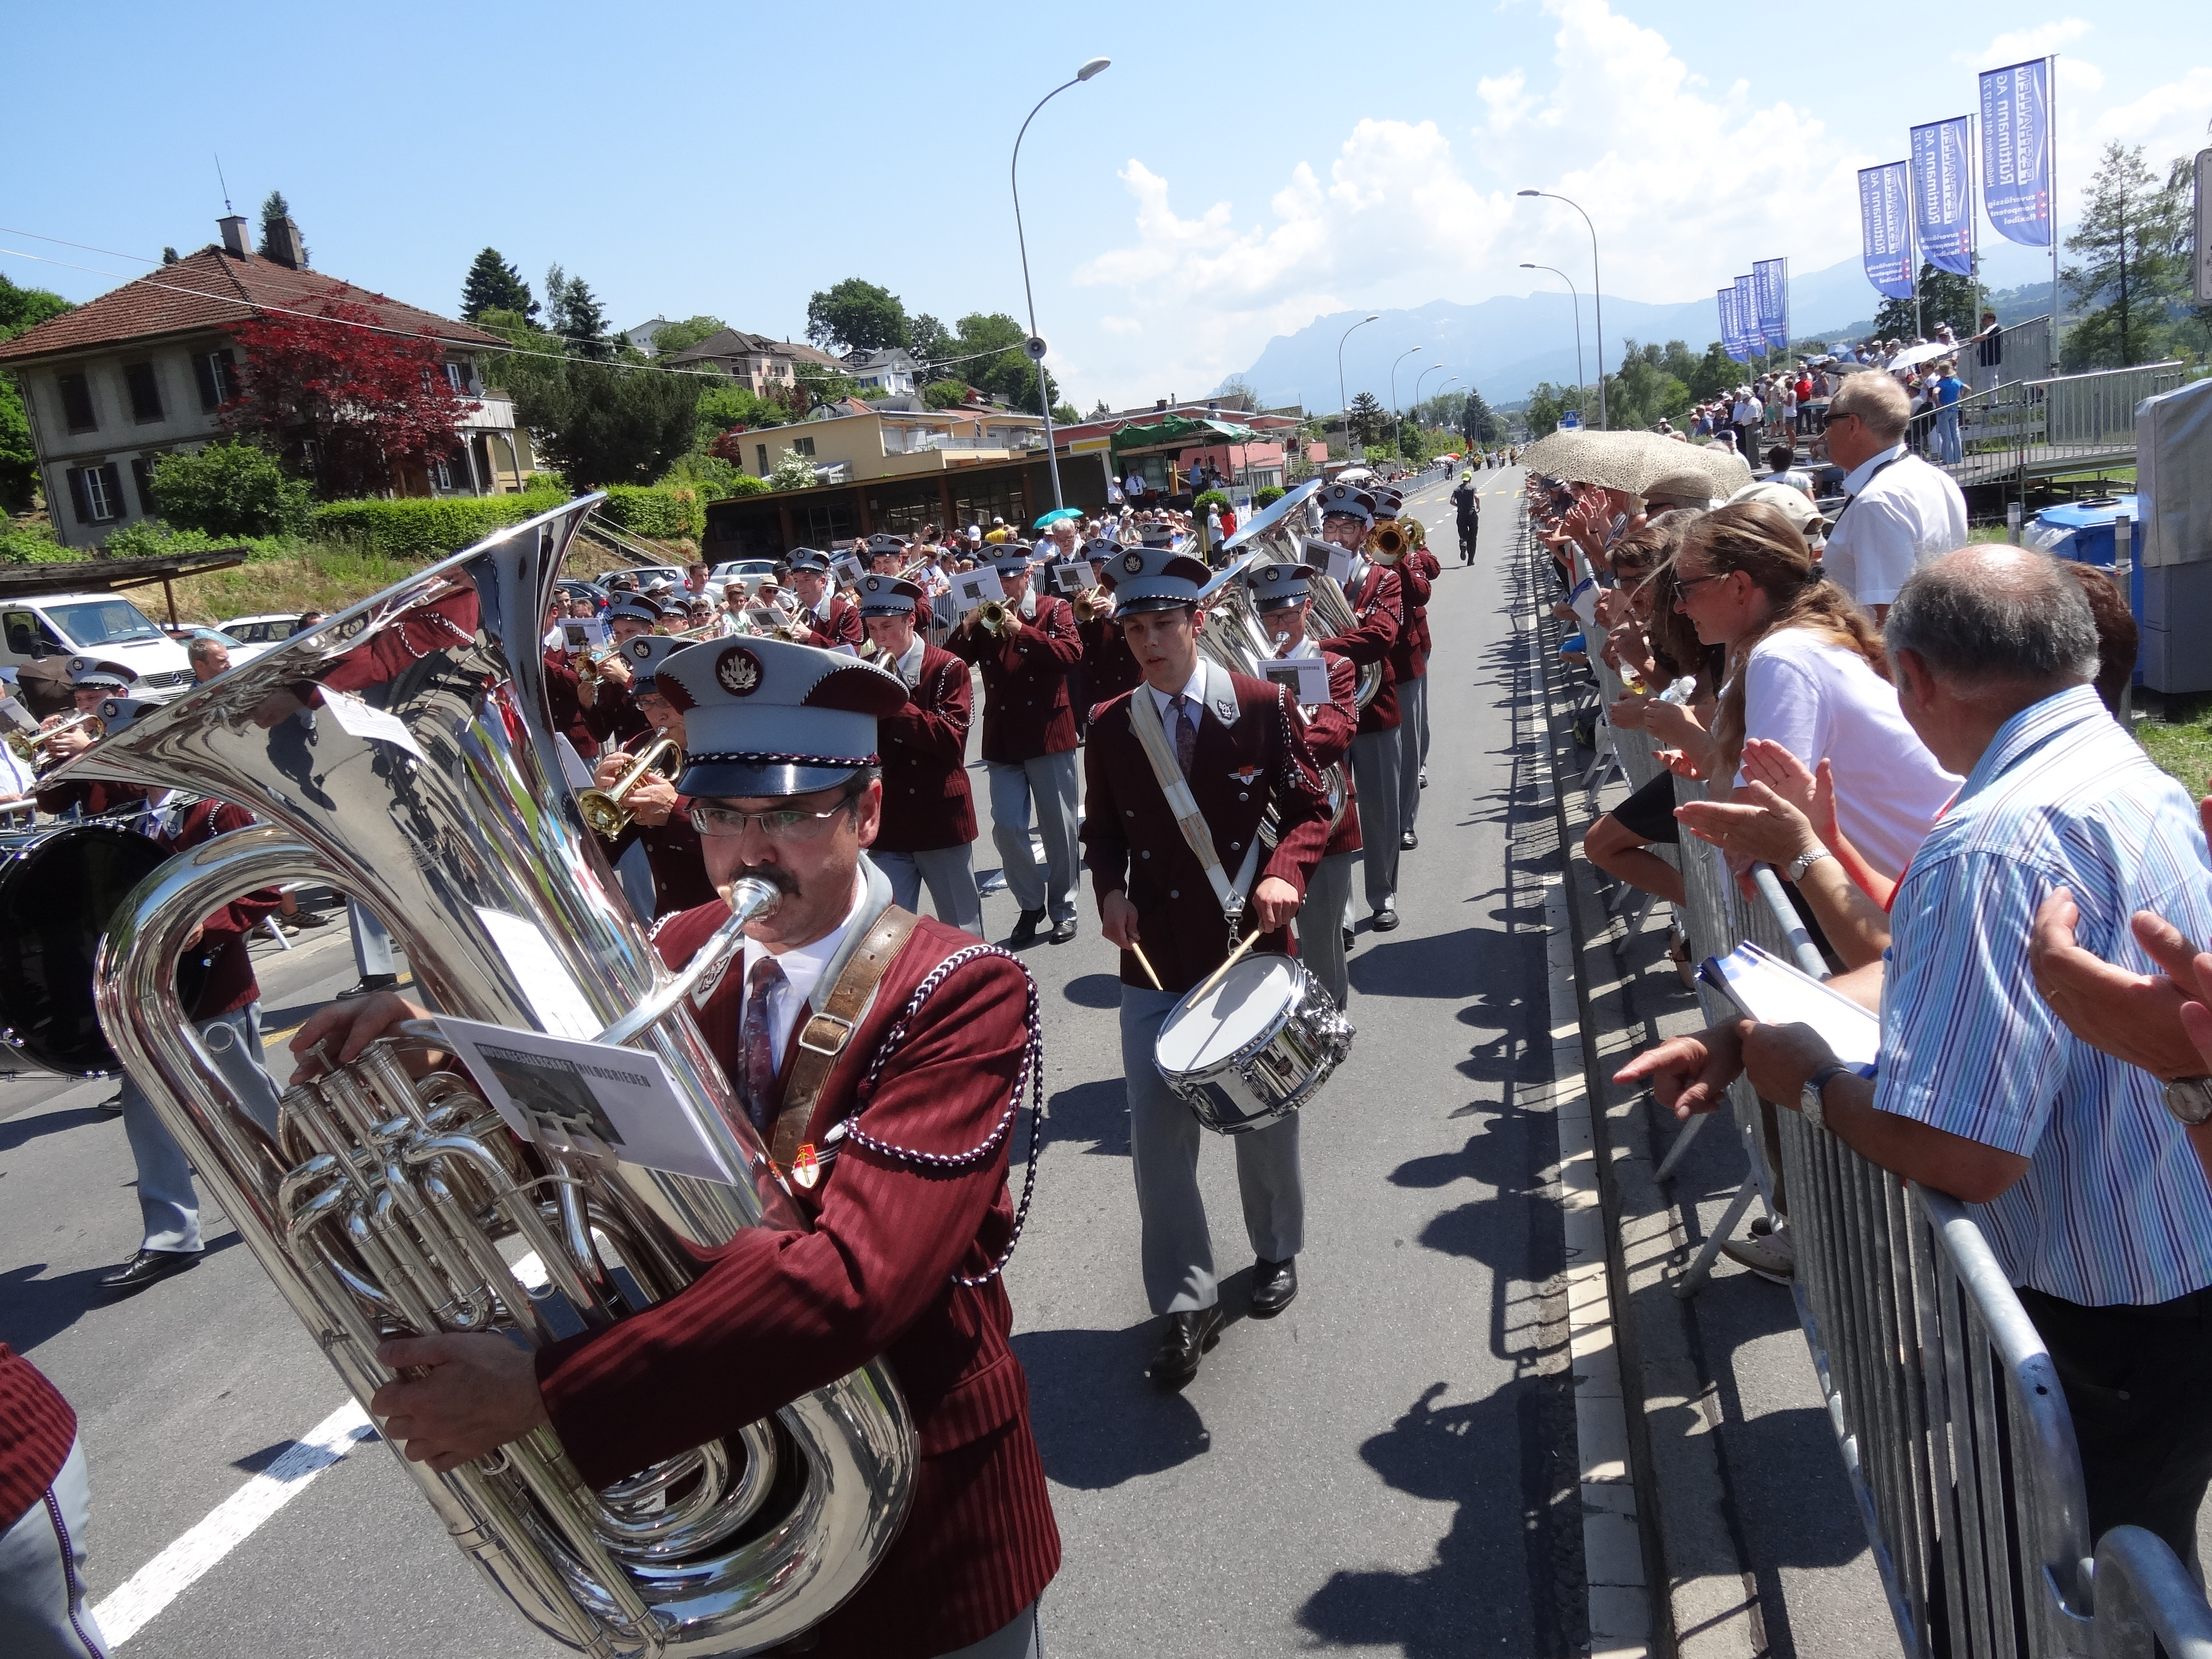
\includegraphics[width=0.85\linewidth]{./chap/2001-2024/2015/Marschmusik-Sempach.jpg}
    \end{MulticolFigure}

    Bei den Vorträgen der Selbstwahlkomposition \enquote{A Malvern Suite} und
    des Pflichtstücks \enquote{Strawabar} konnten wir auf die Unterstützung
    unserer Fans und Musikfreunde zählen, was zu gut gefüllten Rängen und einer
    fantastischen Stimmung führte.

    Trotz eines kleinen Missgeschicks, bei dem ein Solocornetist gezwungen war,
    auf einem Notfall-Ersatzinstrument zu spielen, nachdem er sein eigenes auf
    dem Weg vom Einspielraum zur Festhalle fallen gelassen hatte, fielen die
    Bewertungen der Jury positiv aus.

    Diese Anerkennung spiegelte sich in einem erfreulichen 10. Platz bei der
    Rangverkündigung wider.

    \begin{MulticolFigure}
        \centering
        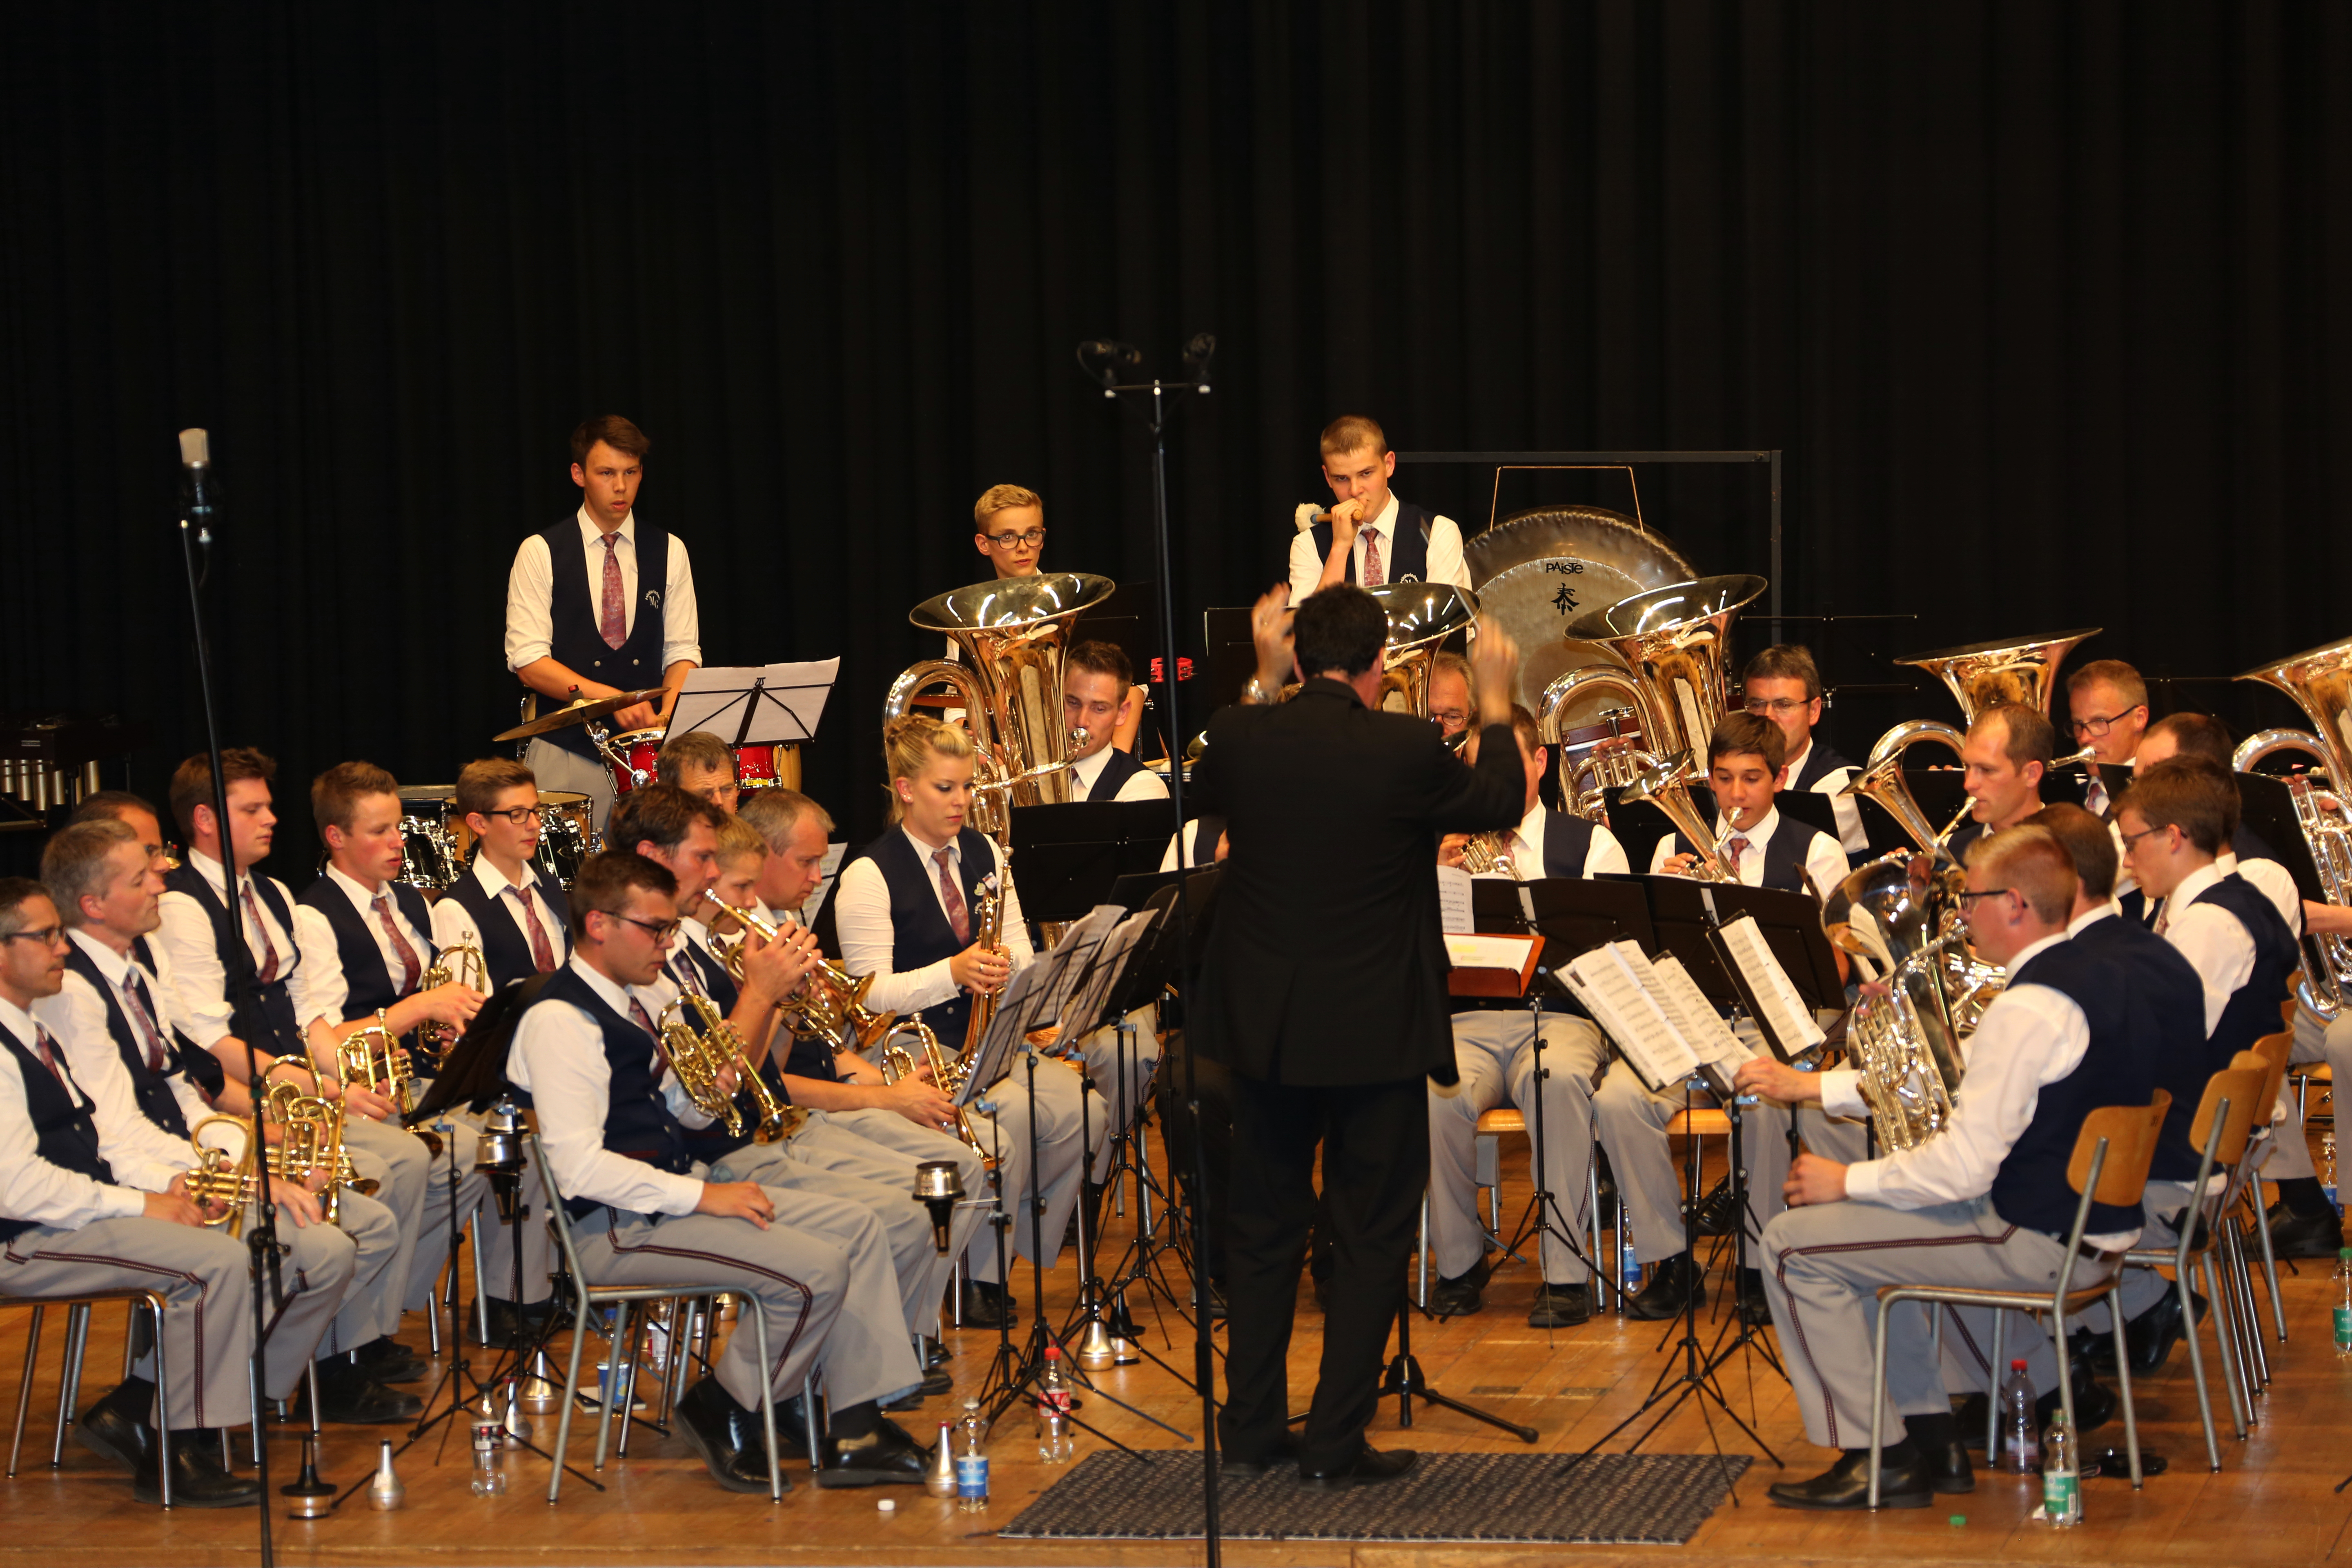
\includegraphics[width=0.93\linewidth]{./chap/2001-2024/2015/Konzertvortrag-Festhalle-Sempach.jpg}
    \end{MulticolFigure}

    Einmal in Fahrt gekommen, konnten sich die Hildisrieder auch am
    anschliessenden Fest und an der Bar nicht aus der Stimmung bringen lassen.
    Daher wurde bis tief in die Morgenstunden eifrig gefestet.

\end{history}


\subsection*{Eidg. Musikfest Montreux, 11. Juni 2016}

\begin{history}


    Das Probewochenende auf dem Hasliberg am 28. und 29. April war der perfekte
    Start in die intensive Vorbereitungsphase für das Eidgenössische Musikfest
    2016. Nachdem alle Instrumente und Ausrüstungen des Schlagregisters sicher
    im Ruagtransporter verstaut waren, reiste der Karavan der Musikgesellschaft
    Hildisrieden problemlos an.

    Im CVJM-Zentrum richteten sie das Quartier kurzerhand als Übungsort her. Das
    gute Wetter zog niemanden nach draussen, sodass die Bedingungen für ein
    produktives Wochenende ideal waren. Die ausgezeichnete Organisation durch
    den Präsidenten trug zu einem reibungslosen Ablauf bei. Insgesamt wurden 15
    Stunden intensiv geübt, nicht eingerechnet die Gesangseinlagen tief in der
    Nacht.

    Die Verpflegung, bereitgestellt von der motivierten Crew der Christlichen
    Vereinigung junger Männer, kam stets pünktlich. Das Wochenende endete ebenso
    problemlos, wie es begonnen hatte, und stärkte sowohl musikalisch als auch
    geistig die Vorbereitung auf das bevorstehende Grossereignis in Montreux.

    Am 20. Mai fand ein Vorbereitungskonzert statt, das von der
    Musikgesellschaft Triengen organisiert wurde. Neben den Gastgebern und den
    Hildisriedern präsentierten auch die Musikgesellschaften aus Rain und
    Schwarzenbach ihre Stücke, die sie über Monate einstudiert hatten. Das
    Konzert offenbarte noch einige musikalische Schwächen, doch der Abend klang
    entspannt an der Bar mit einem kühlen Bier aus.

    Der 26. Mai war der letzte intensive Probetag, bei dem die letzten
    unsicheren Töne aus den Stücken für das Eidgenössische Musikfest entfernt
    wurden.

    Der Höhepunkt der Vorbereitungen war der Auftritt am Eidgenössischen
    Musikfest in Montreux am 11. Juni. Nach einer dreistündigen Fahrt, inklusive
    einer Kaffeepause im Greyerzerland, mussten die Musikanten der MGH sich
    leider ohne die Unterstützung einer Begleitperson auf dem belebten
    Festgelände orientieren.

    Der anhaltende Regen drückte etwas auf die Stimmung, zwang zur Absage der
    frühen Parademusikauftritte und verzögerte den Beginn bis 15:00 Uhr. Doch um
    16:03 Uhr trat die MGH auf und lieferte unter schwierigen wittrigen
    Bedingungen eine beeindruckende Performance ab. Die Jury honorierte ihren
    Marsch \enquote{Geb. Füs. Bataillon 48} von Hans Flury mit hervorragenden 90
    Punkten, was den 2. Platz in unserer Ranglistengruppe bedeutete.

    \begin{MulticolFigure}
        \centering
        \includegraphics[width=0.93\linewidth]{./chap/2001-2024/2016/Marsch-Montreux-2016.jpg}
    \end{MulticolFigure}

    Am Abend präsentierte die MGH das Selbstwahlstück \enquote{Turris
        Fortissima} von Steven Ponsford und das Aufgabenstück \enquote{Caverns}
    von Fabian Künzli vor der Jury, erreichte den 10. Platz und sicherte
    sich so einen Platz in der oberen Hälfte der Rangliste. Die grossartigen
    Erfolge, welche die MGH mit dem Projekt-Dirigenten Pascal Maillard aus
    dem Elsass mit Fleiss, Disziplin und grossem Teamgeist hart
    erarbeiteten, wurden anschliessend an der Riviera von Montreux mit Bier,
    Stumpen und musikalischen Höchstleistungen der Stimmbänder gefeiert. Der
    Bus der MGH verliess als einer der letzten am frühen Sonntagmorgen das
    Festgelände.

    \begin{MulticolFigure}
        \centering
        \includegraphics[width=0.93\linewidth]{./chap/2001-2024/2016/Feiern.jpg}
    \end{MulticolFigure}

    Zum Abschluss des erfolgreichen Musikjahres versammelten wir uns am 17. Juni
    auf dem Bauernhof der Familie Fleischli in St. Anna. Nach einem kurzen
    Marsch genossen die Musikanten ein üppiges Grillfest mit reichlich
    Getränken. Das schöne Sommerwetter hielt leider nicht den ganzen Abend, doch
    das tat der Stimmung keinen Abbruch. Das Dessertbuffet wurde in der
    gemütlichen Stube serviert, und die feierliche Atmosphäre hielt sich bis
    spät in die Nacht. Ein herzlicher Dank geht an die Organisatoren aus dem
    Schlagregister für diesen gelungenen Abschluss.

\end{history}


\groupphoto{0.93}{0.8}{./chap/2001-2024/2016/Montreux-2016.jpg}
{\emph{Eidg. Musikfest Montreux 2016}\\
    1. Reihe: Stephan Wolf, Michaela Balmer, Pascal Maillard, Jonas Furrer,
    Raphaela Balmer\\
    2. Reihe: Franz Dörig, Josef Wolf, Christoph Erni, Peter Estermann, Martin
    Estermann\\
    3. Reihe: Roland Klaus, Christoph Schneider, Manuel Andermatt, Marina
    Büchler, Toni Bachmann\\
    4. Reihe: Fabian Schmid, Mauro Baumann, Daniel Fleischli, Fabian Hüsler\\
    5. Reihe: Elias Troxler, Filip Estermann, Beat Disler, Kilian Rüttimann\\
    6. Reihe: Mattia Klaus, ? Maillard, Florian Koller, André Schmid, Alexander
    Troxler, Stefan Barmet, Dominik Barmet\\
    7. Reihe: Dario Fleischli, Christoph Troxler, Martin Troxler, Jonas Koller,
    Ramon Troxler\\
} {fig:mgh-2016}


\subsection*{Musikantenskirennen Sörenberg, 4. März 2017}

\begin{history}

    Am ersten Märzwochenende fand das alljährliche Musikantenskirennen im
    Sörenberg statt. Neben den zahlreichen Entlebucher Musikanten, waren auch
    einige Hildisrieder unterwegs. Der Vormittag wurde ganz der Rennvorbereitung
    gewidmet. Da die Witterungsverhältnisse nicht den Wünschen entsprach, wurde
    viel Wert auf die mentale Vorbereitung im Restaurant Schwand gelegt.

    Mit Kaffee Luz und einem grossen Mocken Fleisch konnte der Rennhang kurz
    nach Mittag von allen Teilnehmer bewältigt werden. Deren acht waren
    Hildisrieder.

    \begin{MulticolFigure}
        \centering
        \includegraphics[width=0.93\linewidth]{./chap/2001-2024/2017/Skirennen-2017.jpg}
    \end{MulticolFigure}

    Unten im Ziel angekommen gab es wiederum Kafischnaps und perfekte Stimmung
    für ein Skifest. Dieses wurde anschliessend im Gade neben dem Parkplatz
    zusammen mit der Rangverkündigung gehörig gefeiert. Und unter dem Motto
    \enquote{die schnellsten sind nicht immer die Besten} haben die Hildisrieder
    auf ihren Triumph angestossen.


    \subsubsection*{Reise ins Allgäu, 17. und 18. Juni 2017}

    Da die letzte Musikreise schon etwas länger zurückliegt, gönnten sich die
    Musikantin und Musikanten der Musikgesellschaft Hildisrieden mit Begleitung
    am Wochenende vom 17. und 18. Juni 2017 einen Ausflug in das schöne Allgäu
    in Süddeutschland. Am Samstag-Morgen kurz vor 8.00 Uhr versammelte sich die
    Reisegesellschaft bei bestem Wetter vor dem Inpuls, um mit dem Car der Firma
    Estermann Reisen AG pünktlich loszufahren.

    Beim ersten Zwischenhalt in Walenstadt wartete bereits eine Weindegustation
    mit einem \enquote{kalten Plättli} auf die Gruppe. Zu Ehren der kürzlich
    ernannten Veteranen nahmen die Ronspatzen die Instrumente mit und spielten
    zum Ständli auf.

    \begin{MulticolFigure}
        \centering
        \includegraphics[width=0.93\linewidth]{./chap/2001-2024/2017/Ronspatzen.jpg}
        \captionof{figure}{Apéro Ständli der Ronspatzen}
    \end{MulticolFigure}

    Nach dieser gemütlichen und willkommenen Pause ging es weiter nach Sulzberg
    in Österreich. Im dortigen Restaurant Ochsen gab es ein feines Mittagessen
    und es blieb anschliessend genügend Zeit für eine Rundwanderung im schönen
    Gebiet mit Sicht auf die Vorarlberger, wie auch auf die Schweizer Berge.

    Eine weitere Fahrstunde entfernt lag unser Ziel in Kempten. In der
    Brauereigaststätte zum Stift in der Innenstadt nahm die Reisegruppe das
    Nachtessen in Form von feinen, typisch allgäuischen Menus ein. Aber auch für
    die Ohren gab es nochmals einen besonderen Schmaus. Die Ronspatzen hatten
    nämlich die Instrumente nicht nur wegen der Veteranen dabei, sondern vor
    allem aufgrund des kürzlich gewählten Präsidenten des Luzerner Kantonalen
    Blasmusikverbandes, Christoph Troxler, welcher sich sogar noch zu einer
    Soloeinlage hinreissen liess. Die gutgelaunte Gruppe kostete danach voller
    Tatendrang das spätnächtliche Angebot von Kempten aus.

    \begin{MulticolFigure}
        \centering
        \includegraphics[width=0.93\linewidth]{./chap/2001-2024/2017/Reisegruppe.jpg}
    \end{MulticolFigure}

    Um die Stadt auch bei Tageslicht zu Gesicht zu bekommen, gab es am
    Sonntagvormittag noch freie Zeit zur Begutachtung der Sehenswürdigkeiten. Am
    Nachmittag war der Besuch des Skywalk-Naturerlebnisparks in Scheidegg auf
    dem Reiseprogramm. Der Ausblick vom 40 Meter hohen Baumwipfelpfad bot
    einiges und war eindrücklich. Natürlich ist das rustikale Brotzeitbuffet
    noch zu erwähnen, welches zum Abschluss aufgetischt wurde.

\end{history}

\subsection*{Innerschweizer Musikfest Hergiswil, 2019}

\begin{history}

    Wir spielten als erster Verein am Sonntagmorgen, konnten dafür aber schon
    auf der Bühne einspielen. Für das Selbstwahlstück \enquote{Cristo Redentor}
    von Steven Ponsford erhielten wir 93 Punkte, für das gleich darauf folgende
    Aufgabenstück \enquote{Oneiric Tales} von Eddy Debons sogar 94 Punkte.

    Bald zeigte sich, dass wir es auf den 1. Platz der 4 teilnehmenden 2. Klasse
    Brassbands geschafft hatten. Es freute uns besonders, dass wir sogar die BB
    Root geschlagen hatten.

    \begin{MulticolFigure}
        \centering
        \includegraphics[width=0.93\linewidth]{./chap/2001-2024/2019/Marschmusik.jpg}
    \end{MulticolFigure}

    Die Marschzeit war erst am späten Nachmittag geplant. Durch weitere
    Verzögerungen spielten wir schlussendlich erst nach 17.30 den Marsch
    \enquote{Menzberg} von Mario Bürki. Wir bekamen von der Jury dafür 87.3
    Punkte. Das verdiente Bier direkt nach dem Marsch gab es leider nicht, da
    das Bier am Bierstand ausgegangen war.

    \begin{MulticolFigure}
        \centering
        \includegraphics[width=0.93\linewidth]{./chap/2001-2024/2019/Siegerjubel.jpg}
        \captionof{figure}{Siegerjubel}
    \end{MulticolFigure}


\end{history}

\subsection*{Neuuniformierung 2021}

\begin{history}

    Am Sonntag, den 6. Juni 2021, bekamen die Musikanten endliche ihre neue
    Uniform. Ursprünglich war geplant, die Neuuniformierung im September 2020
    durchzuführen. Doch wegen der Covid-19 Pandemie musste die Veranstaltung
    verschoben werden.

    Trotz der immer noch geltenden pandemiebedingten Einschränkungen fand nun
    die Feier in einem angemessenen, wenn auch kleineren Rahmen statt.

    Innovativ beworben wurde dieses Ereignis durch lebensgrosse Pappfiguren,
    anfangs nur in Schwarz und nach der Neuuniformierung in den neuen Uniformen.

    \begin{MulticolFigure}
        \centering
        \includegraphics[width=0.93\linewidth]{./chap/2001-2024/2021/Pappnasen.jpg}
    \end{MulticolFigure}


    \begin{MulticolFigure}
        \centering
        \includegraphics[width=0.93\linewidth]{./chap/2001-2024/2021/Im-Chor-2.jpg}
    \end{MulticolFigure}

    Der Tag begann mit einem würdigen Gottesdienst, in dem unsere neuen
    Uniformen gesegnet wurden.

    \begin{MulticolFigure}
        \centering
        \includegraphics[width=0.93\linewidth]{./chap/2001-2024/2021/Kirchenquartett-1.jpg}
    \end{MulticolFigure}

    Nach dem Gottesdienst folgte ein Fototermin, danach ein gemeinsames
    Mittagessen im Gasthaus Löwen.

    \begin{MulticolFigure}
        \centering
        \includegraphics[width=0.93\linewidth]{./chap/2001-2024/2021/MGH-2021-Gilet.jpg}
    \end{MulticolFigure}

    \begin{MulticolFigure}
        \centering
        \includegraphics[width=0.93\linewidth]{./chap/2001-2024/2021/MGH-2021-lustig.jpg}
    \end{MulticolFigure}

    Am Nachmittag trugen wir verschiedene Ständchen in den neuen Uniformen auf
    dem Schulhausplatz vor, wobei wir uns aus Sicherheitsgründen in drei
    kleinere Gruppen aufteilten, um den COVID-19-Richtlinien gerecht zu werden.

    \begin{MulticolFigure}
        \centering
        \includegraphics[width=0.93\linewidth]{./chap/2001-2024/2021/Ensemble-1.jpg}
    \end{MulticolFigure}

    \begin{MulticolFigure}
        \centering
        \includegraphics[width=0.93\linewidth]{./chap/2001-2024/2021/Ensemble-2.jpg}
        \captionof{figure}{Ensemblekonzerte}
    \end{MulticolFigure}

    \begin{MulticolFigure}
        \centering
        \includegraphics[width=0.93\linewidth]{./chap/2001-2024/2021/Ensemble-3.jpg}
    \end{MulticolFigure}


    Den gelungenen Tag liessen wir mit einem gemütlichen Beisammensein am Abend
    im Löwen ausklingen, wo wir die erfolgreiche Neuuniformierung in kleinem,
    aber feierlichem Rahmen zelebrierten.

    \begin{MulticolFigure}
        \centering
        \includegraphics[width=0.93\linewidth]{./chap/2001-2024/2021/OK.jpg}
        \captionof{figure}{Das OK}
    \end{MulticolFigure}


    Am 25. Juni fand der Abschlussabend der Neuuniformierung statt. Das
    Organisationskomitee, die Ressort-Leiter und die gesamte Musikgesellschaft
    versammelten sich zu einem gemütlichen Abend in der Schüür. Die musikalische
    Untermalung übernahm die Kleinformation Ronspatzen, gefolgt von einem
    exquisiten Abendessen. Es war eine wunderbare Gelegenheit, allen
    Mitwirkenden nochmals herzlich für ihre Beteiligung und Unterstützung zu
    danken.

\end{history}

\groupphoto{1.0}{1.0}{./chap/2001-2024/2021/MGH-2021.jpg}
{\emph{Neuuniformierung 2021}\\
    1. Reihe:\\
    Alissia Schätti, Stephan Wolf, Hans Stöckli, Noe Stadelmann, Franz Dörig,
    Vivienne Bucher, Peter Stadelmann, Lian Wolf, Mattia Klaus, Fabian Hüsler,
    Elia Troxler, André Schmid, Barbara Lingg-Banz\\
    2. Reihe:\\
    Christoph Troxler, Marina Büchler, Robin Estermann, Benedikt Troxler, Filip
    Estermann, Kilian Rüttimann, Beat Disler, Christoph Schneider, Christoph
    Erni, Oliver Schneider, Beat Bachmann, Alexander Troxler\\
    3. Reihe:\\
    Toni Bachmann, Manuel Stirnimann, Yanis Wolf, Jonas Furrer, Stefan Barmet,
    Silvan Wolf, Martin Troxler, Roland Klaus, Peter Estermann, Josef Wolf,
    Stephan Schneider, Mathias Rub } {fig:mgh-2021}


\subsection*{Kant. Musikfest Emmen, 19. Juni 2022}

\begin{history}

    Einige Musikanten hatten sich am frühen Morgen im Omelinger Pool mit einem
    kühlen Bad erfrischt. Nach dem gemeinsamen Morgenessen im Löwen reisten wir
    nach einer kurzen Vorprobe nach Emmen.

    Zuerst mussten wir zur Marschmusik antreten. Da es an diesem Wochenende sehr
    heiss war, warteten wir im Schatten unter der Autobahnbrücke.

    \begin{MulticolFigure}
        \centering
        \includegraphics[width=0.93\linewidth]{./chap/2001-2024/2022/Emmen-Einspielen-unter-Autobahnbrücke.jpg}
        \captionof{figure}{Einspielen im Schatten}
    \end{MulticolFigure}

    \begin{MulticolFigure}
        \centering
        \includegraphics[width=0.6\linewidth]{./chap/2001-2024/2022/Emmen-Marschmusik.jpg}
        \captionof{figure}{Marschmusik bei 35°}
    \end{MulticolFigure}

    Bei über 35° spielten wir den Marsch \enquote{Menzberg} von Mario Bürki. Wir
    bekamen von der Jury 84.8 Punkte. Der dadurch resultierende 1. Rang - den
    wir leider mit Egolzwil teilen mussten - wurde am Abend frenetisch gefeiert.

    \begin{MulticolFigure}
        \centering
        \includegraphics[width=0.93\linewidth]{./chap/2001-2024/2022/Emmen-Gesamtfoto.jpg}
    \end{MulticolFigure}

    Zuvor galt es aber noch, das Selbstwahlstück \enquote{Shine as the Light}
    von Peter Graham und das Aufgabenstück Aufgabenstück \enquote{Cascades} von
    Sami Lörtscher den Juroren zu präsentieren.

    Um nicht in der brütenden Hitze warten zu müssen, versorgten wir uns im
    kühlen Sääli des Restaurants mit Sandwiches. In der extrem heissen Halle
    erreichten beide Vorträge jeweils 90 Punkte, was uns auf den 5. Platz in der
    Rangliste brachte.

\end{history}

\subsection*{Marschpreis.LU, 3. Sept. 2022}

\begin{history}

    Wir spielten den Marsch \enquote{Margam Abbay} von T.J. Powell.

    Unser Transportmittel war ein altes Postauto, und wir begannen den
    Marschpreis in der Mehrzweckhalle Rain. Für unsere Darbietung erhielten wir
    beeindruckende 96 Punkte, was uns in Rain den 2. Platz einbrachte, knapp
    hinter der Kirchenmusik Flühli.

    Unser nächster Auftritt fand auf dem Vorplatz der Halle in Neuenkirch statt,
    wo uns der Juror 92 Punkte zuerkannte. Dies sicherte uns den 4. Gesamtrang
    und wir gewannen zusätzlich den Spezialpreis für die beste Marschbegleitung.

    \begin{MulticolFigure}
        \centering
        \includegraphics[width=0.93\linewidth]{./chap/2001-2024/2022/Einmarsch-Neuenkirch.jpg}
    \end{MulticolFigure}

    Anschliessend ging es weiter zum Knutwiler Bad, wo die Organisatoren eine
    Bühne in einem gedeckten, aber offenen Festzelt errichtet hatten. Der
    Experte war begeistert und vergab 97 Punkte, was uns den 1. Platz vor der
    Kirchenmusik Flühli einbrachte, sowie den Spezialpreis für das am besten
    gespielte Bassteil.

    \begin{MulticolFigure}
        \centering
        \includegraphics[width=0.9\linewidth]{./chap/2001-2024/2022/Knutwil.jpg}
        \captionof{figure}{Knutwil: 97 Punkte}
    \end{MulticolFigure}

    Der letzte Standort war die Lindenhalle in Gunzwil, wo wir erneut starke
    94,5 Punkte erreichten, die jedoch nur für den 6. Platz ausreichten.

    Mit einer Gesamtpunktzahl von 377,5 erreichten wir in der Gesamtwertung den
    2. Platz, knapp hinter der Kirchenmusik Flühli. In der Kategorie 2./3.
    Brassband konnten wir den Sieg erringen.

    Der Preis von 1000 CHF, gesponsert von der Luzerner Kantonalbank, wurde von
    unserem Kassier, der zugleich Vertreter der Bank war, an unseren Präsidenten
    übergeben.

    \begin{MulticolFigure}
        \centering
        \includegraphics[width=0.93\linewidth]{./chap/2001-2024/2022/Preisübergabe.jpg}
        \captionof{figure}{Preisübergabe}
    \end{MulticolFigure}


    \begin{MulticolFigure}
        \centering
        \includegraphics[width=0.93\linewidth]{./chap/2001-2024/2022/Feier-Welle.jpg}
        \captionof{figure}{Freude herrscht}
    \end{MulticolFigure}


    \noindent Folgende Auszeichnungen durfte die MGH entgegennehmen:

    Kategoriensieg Brassband 2./3. Klasse: 1000 Fr.

    Beste Band am Standort Knutwil: 400 Fr.

    Kategoriensieg in Rain und Knutwil: Je 50 Fr.

    Spezialpreis für das bestgespielte Bassteil: 1 Fässli Bier

    Spezialpreis für die beste Marschbegleitung: 5 Liter Magnum Weinflasche


    \subsubsection*{Vereinsreise ans Musikprob Brassfestival Pullendorf DE, 2. und 3. Sept. 2023}

    Am Morgen fuhren wir los mit dem Car und stärkten uns bei der Raststätte
    Kempthal noch für den weiteren Tag, dann fuhren wir weiter nach Pfullendorf.

    Nach dem Einchecken nahmen wir am Brassfestival Musikprobe teil, bei dem wir
    grossartige Brass-Musik geniessen und das eine oder andere Bierchen nehmen
    konnten.

    Am nächsten Morgen fuhren wir mit etwas kleinen Augen mit dem Schiff nach
    Konstanz. Spätestens da war es von Vorteil, dass der Magen bei allen wieder
    in Ordnung war. Ein paar Stunden konnten wir dann in Konstanz verweilen,
    bevor wir uns bereits wieder auf den Rückweg machten.

    Nochmals ein herzliches Dankeschön an die zwei Organisatoren Silvan und Max.
    Es war ein absolut hammermässig gut organisierter Ausflug. Gefeiert haben
    die zwei das bereits am 4. Januar ausgiebig im Löie und in der LTH Bar
    unten. Details kenne ich nicht, aber am besten geht ihr direkt zu den
    Organisatoren und fragt nach.


\end{history}
